%\begin{itemize}
%    \item
%        Weshalb wurde das benutzte mathematische Modell gew\"ahlt?
%    \item
%        Weshalb wird ein Schaltregler benutzt?
%    \item
%        Weshalb wurde ein eigenes PCB entwickelt statt ein Steckbrett verwendet?
%    \item
%        Wie soll unser Ger\"at bedient werden k\"onnen?
%\end{itemize}

Underpinning  our  device  is  a  microcontroller which  has  as  its  primary
responsibilities the  handling of IO tasks  (such as user interaction  and the
display) and  controlling the step-down converter. Power  delivery is realised
with a prebuilt DC power supply unit as per the requirements.

With  an  eye towards  potential  serial  production,  a proprietary  PCB  was
developed.  This allows tight control  over impedances in the lines connecting
critical  components and  brings the  behavior  of the  prototype device  much
closer  to  a mass  produced  version  than  a breadboard  solution  could. It
should  also  be  pointed  out  that  trace  routing,  lengths  and  component
placement are crucial,  as is discussed in  section \ref{sec:verification} (p.
\pageref{sec:verification}ff), \emph{Verification}.

Interaction with  our device can  be done both  via physical interface  on the
device itself,  which is comprised  of a display  and a push-twist  button, as
well as  on a PC  connected by USB  using our software  \emph{Smooth} (section
\ref{subsec:frontend}, p. \pageref{subsec:frontend}ff).


% **************************************************************************** %
\subsection{Concept of Regulation Circuit}
% **************************************************************************** %

\begin{minipage}{0.5\textwidth}
    \center
    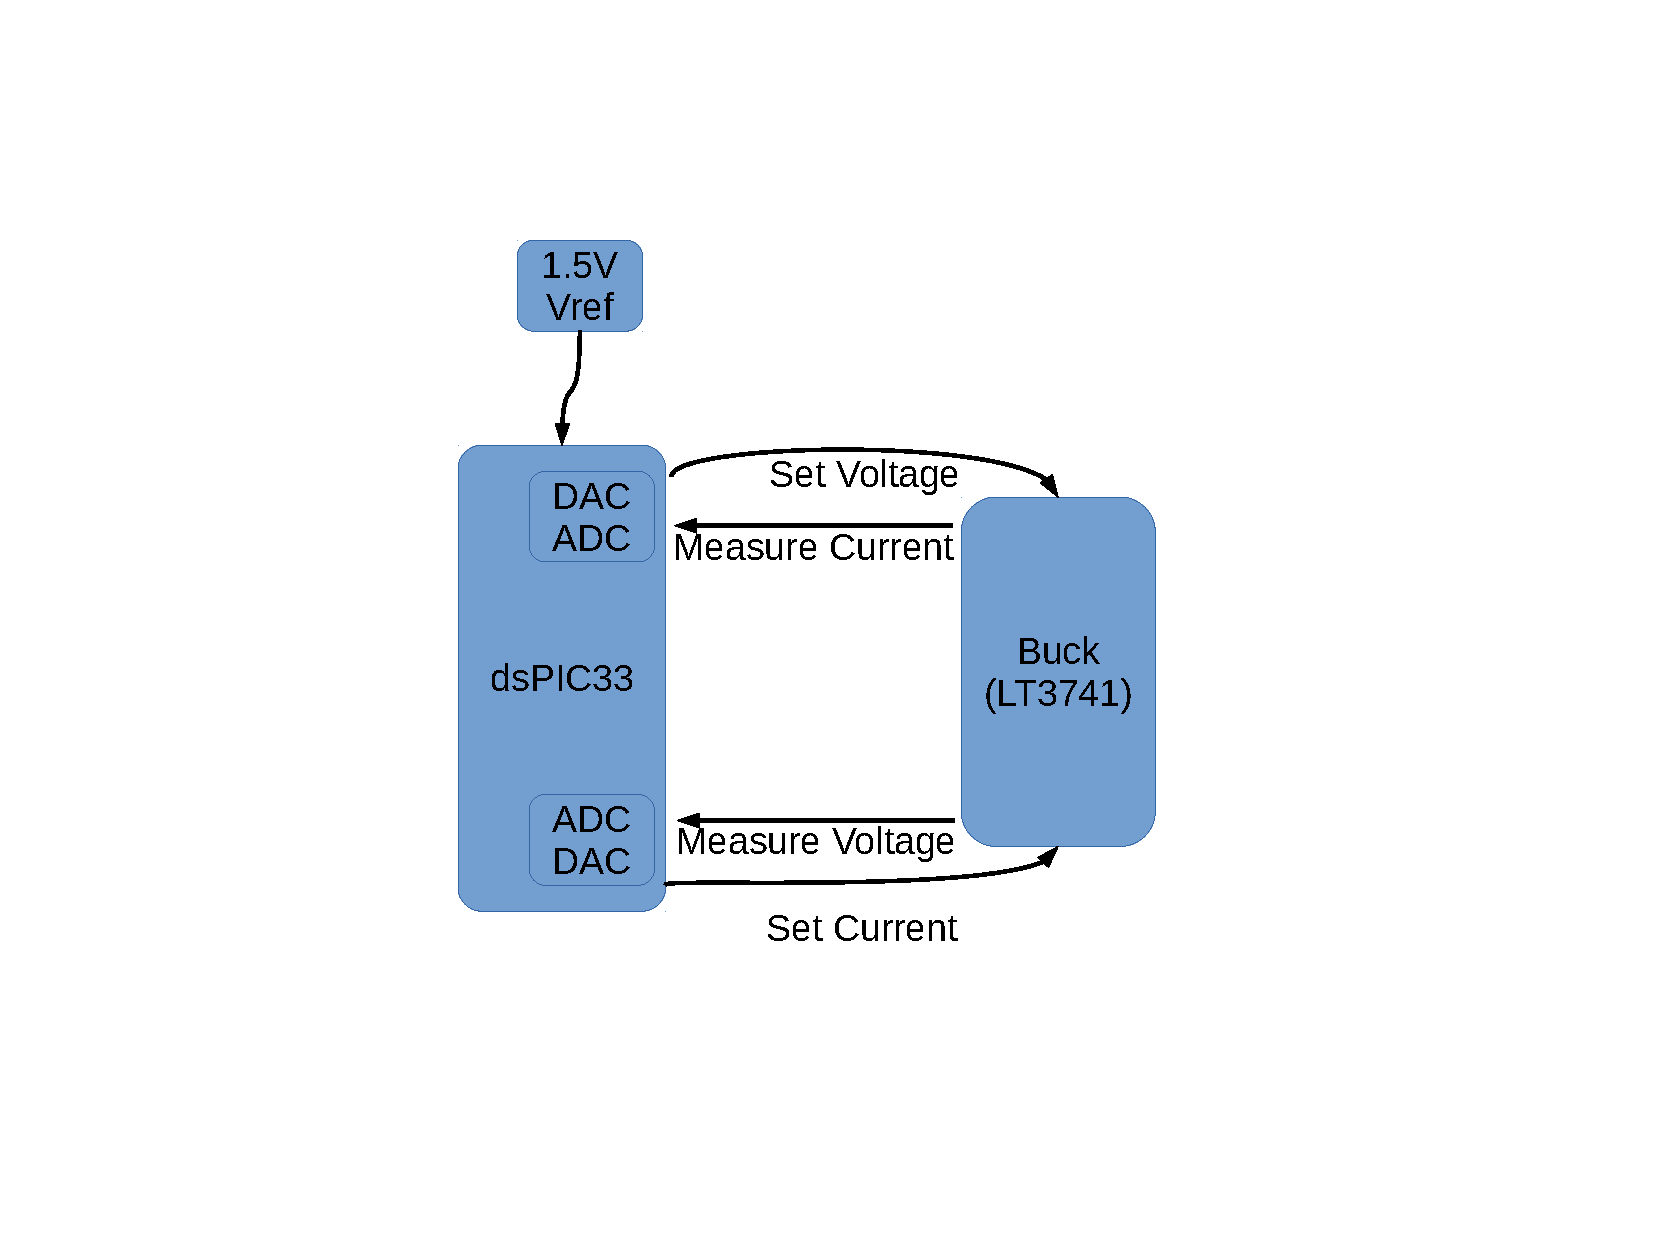
\includegraphics[width=\textwidth,trim=140 140 120 100,clip]{images/block-diag-control.pdf}
    \captionof{figure}{Block diagram of control circuit}
    \label{fig:diag:block}
\end{minipage}
\begin{minipage}{0.5\textwidth}
    \center
    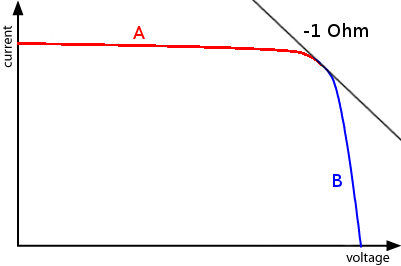
\includegraphics[width=\textwidth]{images/vi-curve.png}
    \captionof{figure}{VI-Curve with \SI{-45}{\degree} slope indicated}
    \label{fig:circuit:buck:uset}
\end{minipage}


\subsection{Goals of the model}

Our aim is to have a simple model, as usability is more important than accuracy.
In  other words, our model should have a small set of parameters, which  can  be
easily determined by the  user. Further it must respect solar irradiation, as we
want  to  model  how clouded skies or a partially  covered  module  affects  its
output.


\subsection{Model for one solar cell}

As Basis for our model serves the single diode model of  the  ideal PV cell from
\cite{ref:villa:pvmodel} \todo{make references work} . The I-V characteristic of
this circuit is
\begin{equation} \label{eq:IV_old}
 I = I_{pv} - I_o \left[ \exp \left( \frac{V}{V_T} \right) - 1 \right]
\end{equation}
where $I_{pv}$ is the generated current, $I_o$ is the diode current and $V_T$ is
the thermal voltage. All of these three parameters are dependent on the junction
temperature, however to simplify our model  we  assume  that  the temperature is
equal to the nominal temperature $T_n = 298.15K$. The thermal voltage is defined
with
\begin{equation}
    V_T = a k T / q
\end{equation}
where $T$ is the junction Temperature,  $k$ is the boltzman-constant, $q$ is the
electron charge constant and $a$  is  the  diode  ideality  factor,  which  lies
usually around 1.2 for silicium substrates. This  gives  us $V_T \approx 30.8mV$
for one cell. The current generated by the cell is defined as
\begin{equation}
    I_{pv} = \left( I_n + K_I \Delta_T \right) \frac{G}{G_n}
\end{equation}
with  $I_n$  being  the  nominal  Current  and  $G$  and $G_n$ being the  actual
respectively  the nominal solar irradiation. For our  model  we  will  set  $I_n
\approx I_{sc}$ and again assume that $T  =  T_n$ giving us $\Delta_T = 0$ which
simplifies this formula to
\begin{equation} \label{eq:I_pv}
    I_{pv} = I_{sc} \frac{G}{G_n}
\end{equation}
Finally, the  diode  leakage  current  at  the nominal temperature \footnote{For
other temperatures please see \cite{ref:villa:pvmodel}} is
\begin{equation} \label{eq:I_o}
    I_o = \frac{I_{sc}}{e^{V_{oc} / V_T} - 1}
\end{equation}
If we put \eqref{eq:I_o} and \eqref{eq:I_pv}  back  in  \eqref{eq:IV_old} we get
\begin{equation}
    I = I_{sc} \left( \frac{G}{G_n} - \frac{e^{\frac{V}{V_T}}-1}{e^{\frac{V_{oc}}{V_T}}-1} \right)
\end{equation}
If we now assume $V_{oc} >  5  *  V_T$ we can say that $e^{\frac{V_{oc}}{V_T}}-1
\approx e^{\frac{V_{oc}}{V_T}}$ and our final formula becomes
\begin{equation} \label{eq:IV}
    I = I_{sc} \left( \frac{G}{G_n} - e^{\frac{V - V_{oc}}{V_T}} \right)
\end{equation}


\subsection{Model for multiple Cells in Series}

If  the  solar irradiation is the same for every cell in series, then the  whole
array  can  also  be  simulated  with  \eqref{eq:IV}, but $V_{oc}$ and $V_T$ get
multiplied by the number of cells.

If  the  irradiation isn't the same for all cells, for instance because one cell
is shaded, a more complex model must be used.
\begin{figure}[h]
	\center
    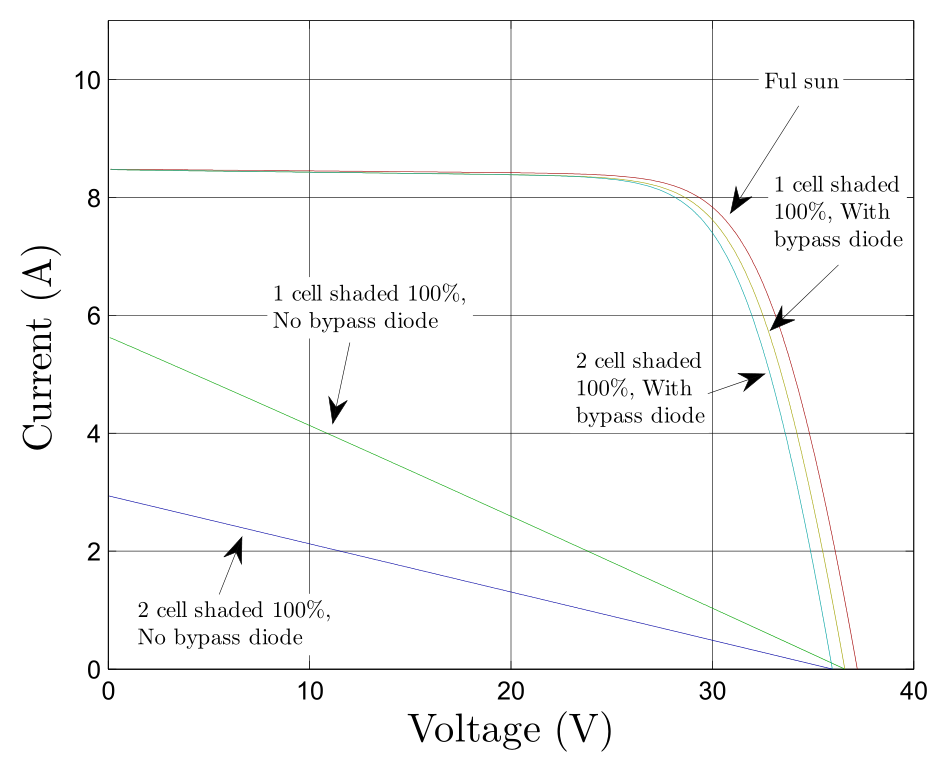
\includegraphics[width=.5\textwidth]{images/model/shaded.png}
    \caption{I-V curves for different configurations and shaded cells\cite{ref:tian:model}}
    \label{fig:model:shaded}
\end{figure}

Figure \ref{fig:model:shaded} shows how  varied  the characteristics of a shaded
PV-module can be and how bypass diodes affect them. In our model  we can imitate
the I-V curve of an array with a shaded cell and no bypass diode by setting $V_T
= V_{oc}$.

\begin{figure}[h]
	\center
    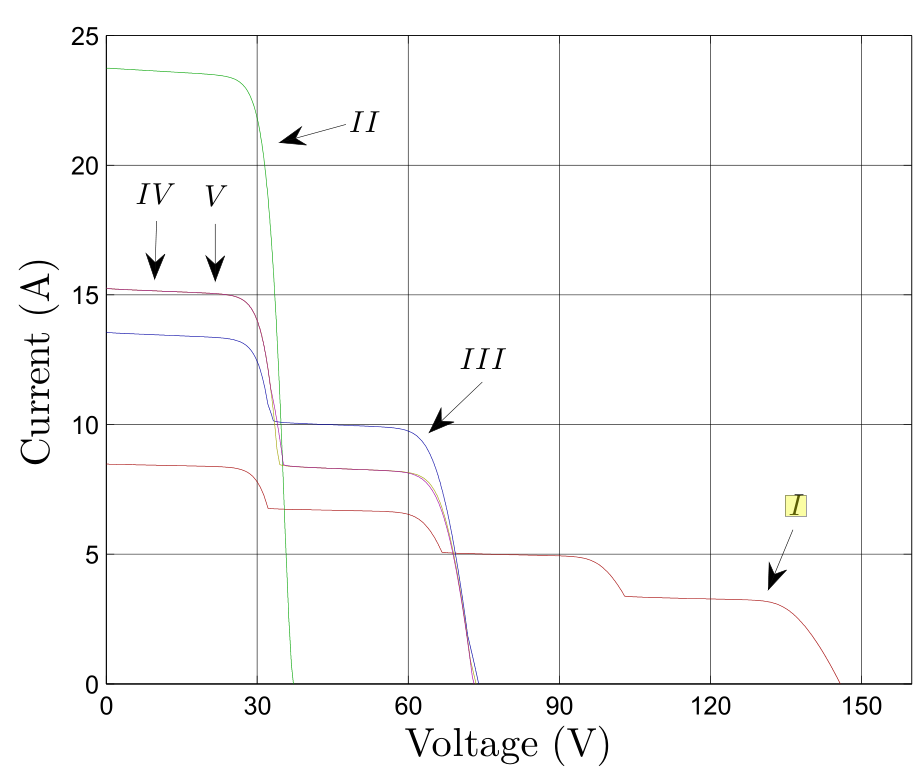
\includegraphics[width=.5\textwidth]{images/model/steps.png}
    \caption{The typical characteristic of modules connected in series or in parallel}
    \label{fig:model:steps}
\end{figure}
The "stairway" \todo{fix} characteristic shown  in  figure \ref{fig:model:steps}
emerges  when  two or more modules, which are exposed to different  irradiation,
get connected in series with bypass diodes. To simulate this behaviour,  we take
a  number of curves with decreasing short circuit current  and  increasing  open
circuit  voltage  and determine which curve is applicable by checking what curve
returns the maximum current for the given voltage.

